\documentclass[a4paper,11pt]{article}

\usepackage[utf8]{inputenc}
\usepackage[a4paper, left=3cm, right=3cm, top=3cm, bottom=3cm]{geometry}
\usepackage[frenchb]{babel}
\usepackage{default}
\usepackage{pslatex}
\usepackage{graphicx}
\usepackage{algorithmic}
\usepackage{multicol}
\usepackage{amsmath}
\usepackage{amssymb}
\usepackage{textcomp}
\usepackage{pgf}
\usepackage{pgfplots}
\usepackage{tikz}
\usepackage{pgfplots}
\usepackage{capt-of}
\usepackage{esvect}
\usepackage[T1]{fontenc}
\usepackage[babel=true]{csquotes}
\usepackage{gensymb}
\usepackage{listings}

% \setcounter{tocdepth}{4}

%opening
\title{Tropodrone}
\author{Thibaut Manceau, Alexis Gros, Noé Gueydan, Tristan Porteries}

\begin{document}

\begin{Huge}
\maketitle
\end{Huge}

\clearpage

\tableofcontents

\clearpage

\section{Introduction}

\subsection{Besoins}
Notre projet part d'un constat: Les drones sont amenés à se développer fortement dans les années à venir, par exemple avec les services de livraison d'Amazon. Dans ce cadre, nous voulions apporter une amélioration significative pour répondre aux problématiques suivantes:
\begin{itemize}
	\item Autonomie: \\
		Les drones, particulièrement les drones quadricoptères de petite envergure possèdent une assez faible autonomie, ce qui réduit leur rayon d'action ainsi que la charge utile qu'ils peuvent supporter.
	\item Sécurité: \\
		Les drones sont des dangers, pour eux mêmes comme pour leur environnement. Les drones peuvent souffrir de problèmes techniques (comme la perte de batterie) et tomber en vol. On devine les dangers inhérents à ce genre de situation. De plus, les drones rentrent parfois dans des obstacles, et les dégâts peuvent vite revenir cher.
\end{itemize}

\subsection{Notre projet}
Notre projet part de ces constats pour aboutir à une solution, novatrice, qui n'a pas de concurrence sur le marché~: proposer aux pilotes amateurs et aux industriels un hybride entre un drone et un petit dirigeable à travers une structure qui permette d'augmenter un petit drone quadricoptère de 25 cm d'envergure.

\subsection{Contraintes}
Nous avons défini des besoins, de ces besoins découlent des contraintes. Ces contraintes sont:
\begin{itemize}
	\item Autonomie~:
		\begin{itemize}
			\item Du drone~:\\
			Avoir une autonomie supérieure à celle du drone, avec comme sans charge utile.
			\item Des ballons~:\\
			Avoir des ballons "étanches" à l'hélium, c'est à dire qui le retiennent au moins trois jours avec des pertes de l'ordre de 30\%.
		\end{itemize}
	\item Sécurité~:
		\begin{itemize}
			\item Structure~:\\
				Faire une structure qui enveloppe le drone et le protège des chocs.
			\item Sustentation~:\\
				Éviter que le drone ne tombe de manière dangeureuse en cas de problème technique.
		\end{itemize}
	\end{itemize}
	Afin que le drone reste manoeuvrable malgré sa structure, nous nous sommmes également fixé des contraintes de manoeuvrabilité~:
	\begin{itemize}
		\item Maneuvrabilité~:
			\begin{itemize}
				\item Retenir le drone~:\\
					La structure doit entacher au minimum les déplacements possibles du drone, en rotation comme en translation.
				\item Navigation~:\\
					Le drone doit pourvoir naviguer sur un interval de 15 mètres de hauteur.
			\end{itemize}
	\end{itemize}

\subsection{Applications}
Pour répondre à ses contraintes, nous avons mis en place ces solutions:
\begin{itemize}
	\item Ballons~:\\
		Nous utilisons trois ballons de 25m3 de contenance pour retenir le poids d'un drone de 750g, ce qui permet de très fortement ralentir sa chute.
	\item Structure~:
		\begin{itemize}
			\item Les ballons sont positionnés de sorte que leur centre de gravité coïncide avec celui du drone, pour plus de stabilité~;
			\item Le drone est relié à la structure par deux fils, ce qui lui laisse une grande liberté de mouvements~;
			\item Les ballons, disposés autour du drone, le protègent des chocs.
		\end{itemize}
\end{itemize}


\subsubsection{Légalité}
Faute de juridiction quant aux appareils volants de ce type, nous nous sommes rabattus sur les contraintes légales imposées aux drones et aux ballons séparément.\\
\begin{itemize}
	\item Notre drone est de catégorie A (- de 25 kg)~:\\
		Il n'est soumis à aucune contrainte qui nous limiterait dans le choix de nos solutions techniques, ou qui limiterait nos objectifs.
		Cependant, nous restons soumis aux mesures de sécurité élémentaires (ne pas trop s'approcher durant la phase de décollage et d'atterissage, ne pas survoler les terrains militaires...).
	\item Le ballon entre dans la catégorie « léger »~:\\
		La ficelle supportant la charge utile doit casser au-dessous de 23 kg.
		Suite à des tests, la ficelle qui servira à tenir nos ballons se rompt à une tension comprise entre 15 et 20 kg.
\end{itemize}

\subsubsection{Drone}
\begin{multicols}{2}
	Drone XCSOURCE~: \\
	\begin{itemize}
		\item 290 mm diagonale~;
		\item 190 mm longueur~;
		\item 70 mm hauteur~;
		\item moteur EMAX MT2204 2300KV Brushless Motor~;
		\item Accu Lipo Gens Ace 2200Mah 11.1V 25C 3S~;
		\item 450 g.
	\end{itemize}
	\begin{center}
		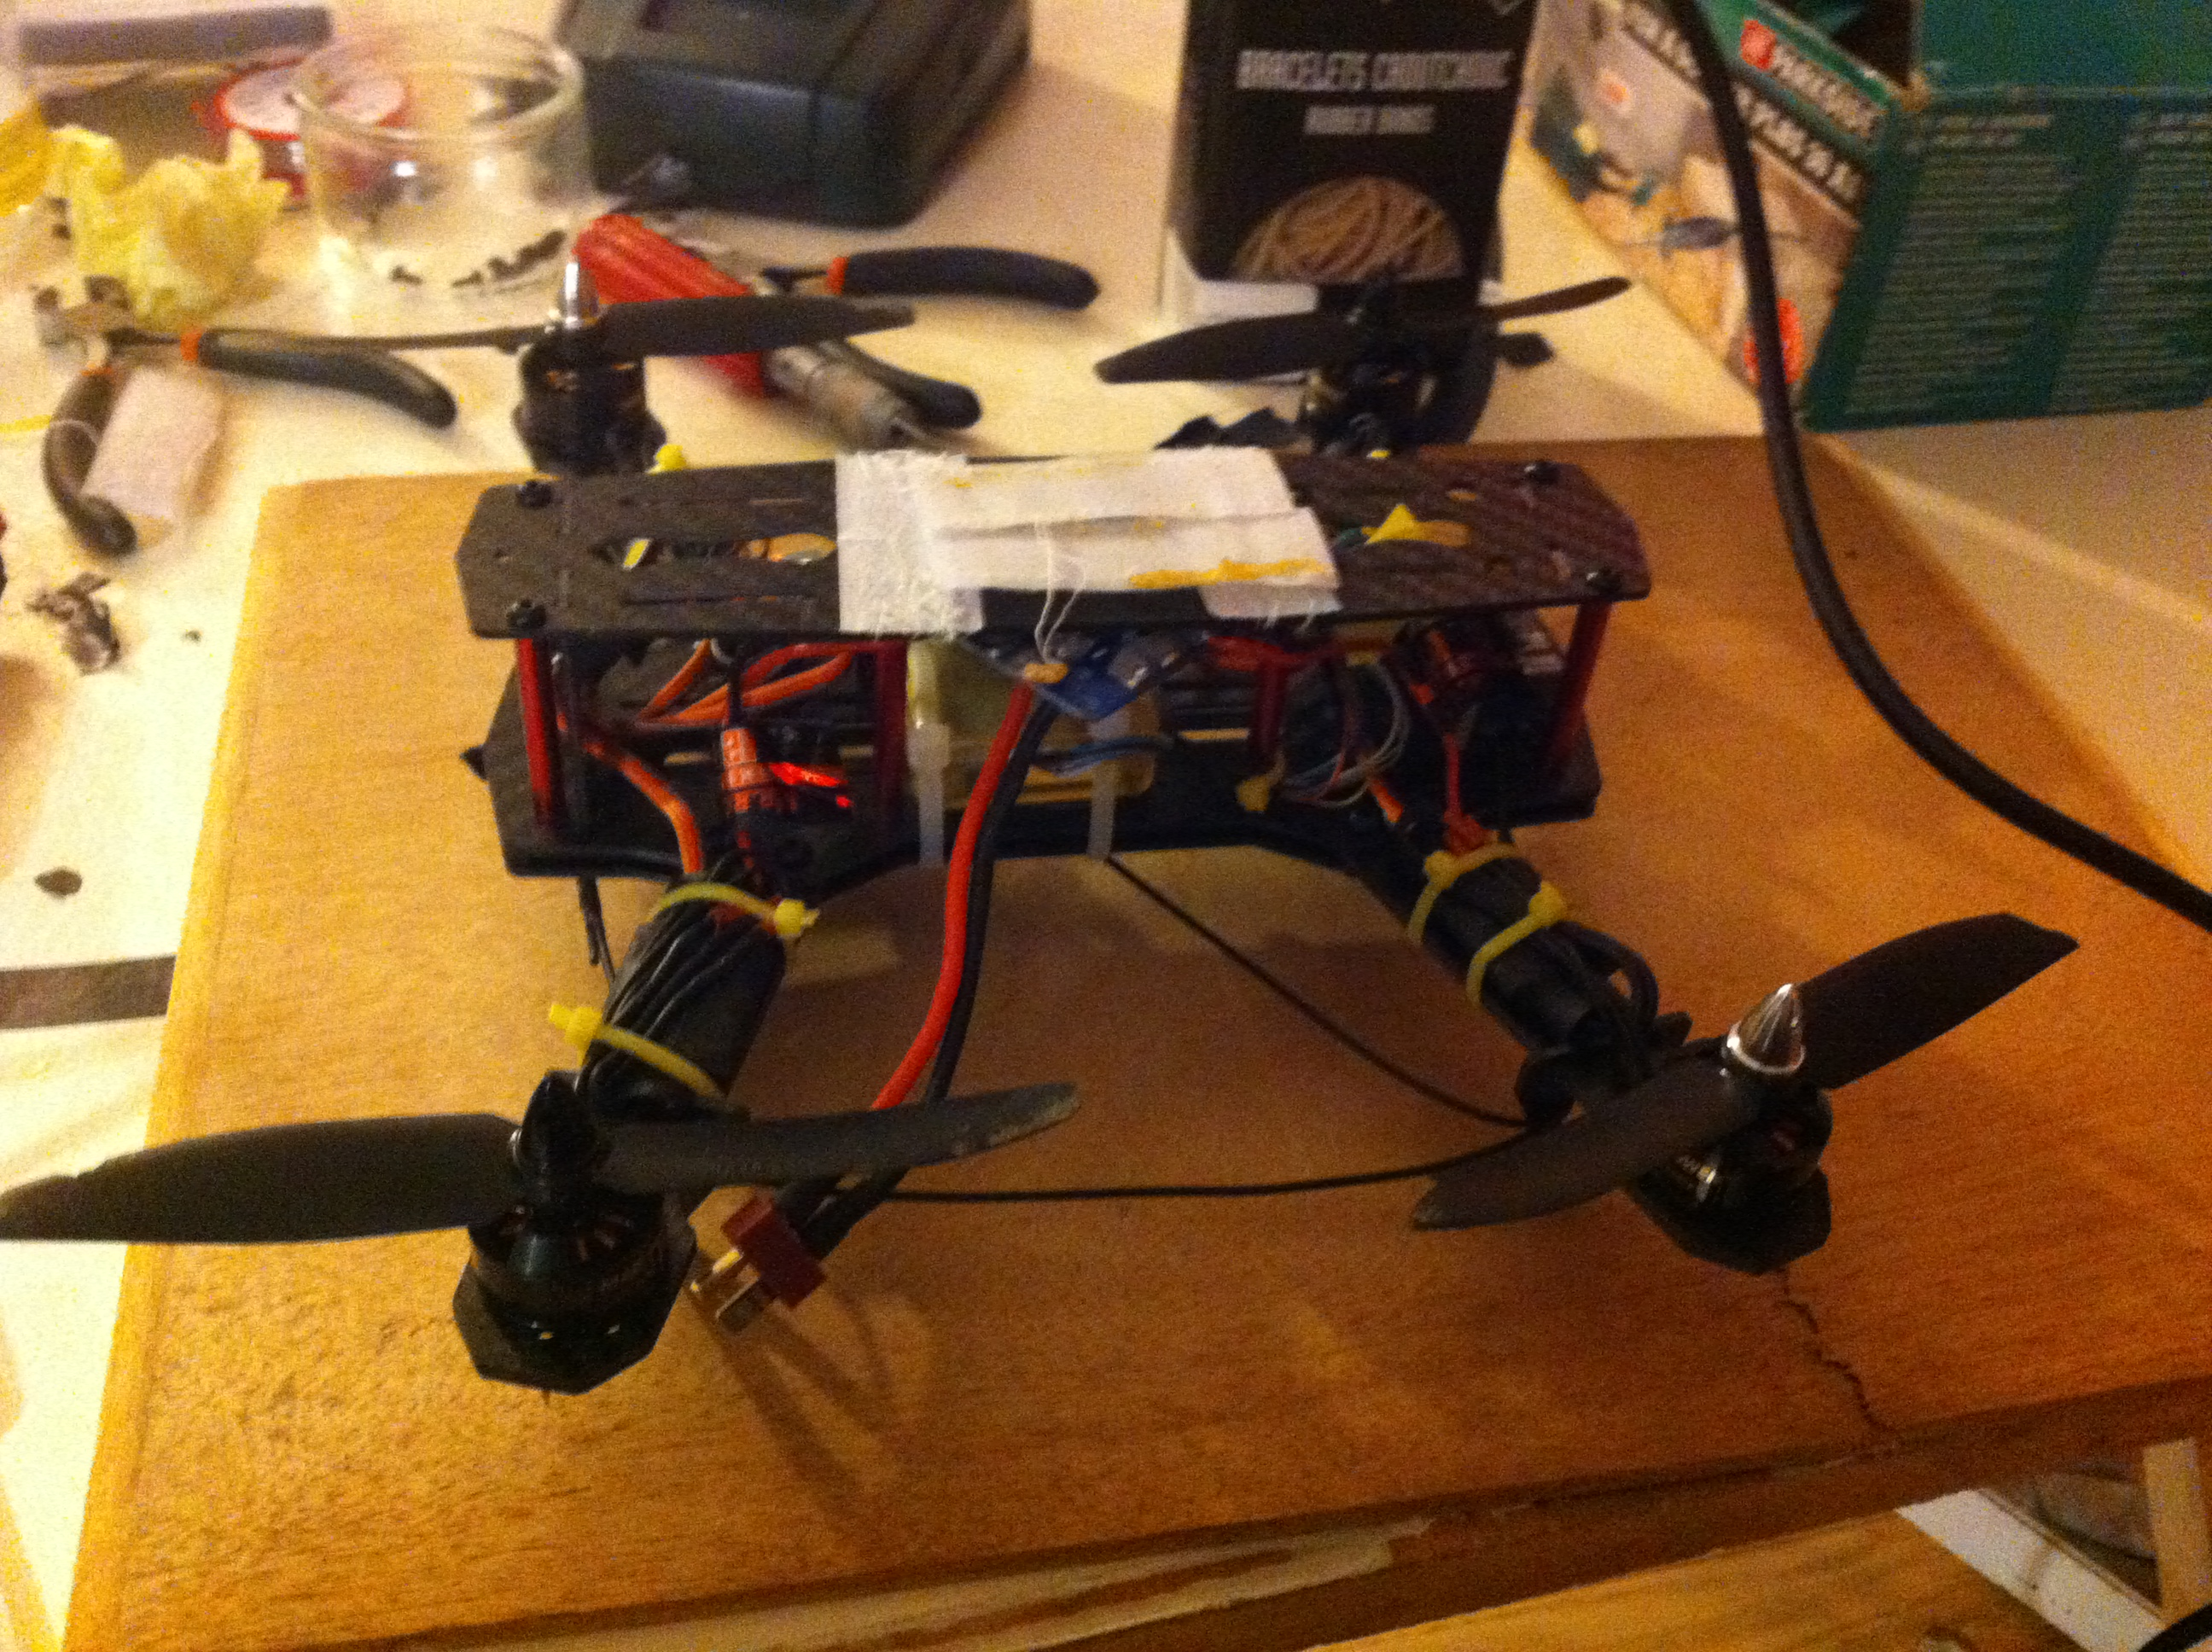
\includegraphics[width=6cm]{../Images/drone.JPG}
	\end{center}
	\captionof{figure}{Drone XCSOURCE.}
\end{multicols}

\newpage

\section{Étude de conception}

\subsection{Ballon}

\subsubsection{Élévation}

Le tropodrone doit utiliser un moyen de supporter une partie du poids du drone sans dépenser d'énérgie dans le but d'augmenter l'autonomie, pour ce faire nous utilisons la poussée d'Archimède d'un gaz plus léger que l'air. Comme ce gaz est plus léger que l'air la somme de son poids et de sa poussée d'Archimède forment une force verticale orienté vers le haut.

\paragraph{Archimède}

La poussée d'archimède est définie par~:

\enquote{Tout corps plongé dans un fluide au repos, entièrement mouillé par celui-ci ou traversant sa surface libre, subit une force verticale, dirigée de bas en haut et opposée au poids du volume de fluide déplacé ; cette force est appelée poussée d'Archimède.}

\begin{center}
	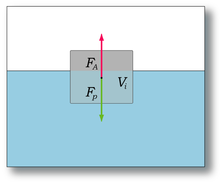
\includegraphics[width=5cm]{../Images/pousse_archimede.png}
\end{center}

Cette force se calcule avec la formule~:

\begin{center}
  \boxed{\vv{Fa} = -M_F \times \vv{g}}
\end{center}

Où $\vv{Fa}$ est la poussée d'archimède en $N$, $M_F$ la masse du fluide contenue dans le volume déplacé en $kg$, $\vv{g}$ la valeur du champ de pesanteur en $N.kg^{-1}$. \\

Un ballon de gaz est donc soumis à deux forces~: son poids et sa poussée d'Archimède~:

\begin{center}
  \boxed{\vv{F_{ballon}} = \vv{P_{ballon}} + \vv{Fa_{ballon}}}
\end{center}

Où $\vv{F_{ballon}}$ est la force d'élévation du ballon en $N$, $\vv{P_{ballon}}$ le poids du ballon en $N$, $\vv{Fa_{ballon}}$ la poussée d'Archimède éxercée sur le ballon en $N$. \\

Nous pouvons remarquer que si $P_{ballon} < Fa_{ballon}$ alors il existe une force d'élévation orienté vers le haut. De même cette force sera toujours  plus petite que la poussée d'Archimède éxercée sur le ballon, comme le ballon et le gaz possède toujours une masse~: $F_{ballon} < Fa_{ballon}$.
Par la suite nous appellerons capacité d'élevation la masse que peut supporter la force d'élévation d'un ballon~:
\begin{center}
	\boxed{Ca_{ballon} = \frac{F_{ballon}}{g}}
\end{center}

Où $Ca_{ballon}$ est la capacité d'élévation en $kg$, $F_{ballon}$ la force d'élévation en $N$ et $g$ la valeur du champ de pesanteur en $N.kg^{-1}$.

\paragraph{Gaz}

Pour avoir un gaz plus léger que l'air il faut qu'il est une masse volumique inférieur à celle de l'air~: $1.29kg.m^3$. Plusieurs gazs remplissent cette condition, les plus courants sont l'hélium est l'hydrogène dont les masse volumique et les capacités d'élévation calculées sont~:

\begin{center}
	\begin{tabular}{|l|c|c|c|}
		\hline
		Gaz & Air & Hydrogène & Hélium \\
		\hline
		Masse Volumique $(kg.m^3)$ & 1.29 & 0.08988 & 0.1785 \\
		\hline
		Force d'élévation $(N.m^3)$ & 0 & 11.77 & 10.90 \\
		\hline
	\end{tabular}
\end{center}

Le gaz retenu et l'hélium car il ne présente pas de rique de combustion contrairement à l'hydrogène, même si sa masse volumique est plus importante et que sa procuration est plus compliquée.

\paragraph{Dilatation}

En prenant exemple sur les montgolfières nous avons cherché à connaitre le gain de volume que pourrait avoir l'hélium à une température élevée. Ce gain de volume apporte directement une reduction de la masse volumique et donc l'augmentation de la force d'élévation.

La loi de Charles permet de calculer la dilatation d'un gaz. D'après Charles il existe un rapport volume température constant dépendent seulement de la pression du gaz et de la quantité de matière du gaz étudié.

\begin{center}
 \boxed{\displaystyle{\frac{V_1}{T_1} = \frac{V_2}{T_2} = f(P, n)}} \\
 $\displaystyle{V_3 = f(P, n) \times T_3}$
\end{center}

Où $V_n$ est le volume du gaz en $m^3$ à la température $T_n$ en $K$, $P$ la pression du gaz en $Pa$, $n$ la quantité de matière en $mol$ et $f(P, n)$ le rapport constant entre volume et temperature en $m^3.K^{-1}$.

L'application de cette loi à l'hélium à une température de $200 \degree C $ donne les résultats suivants~: \\

Le volume molaire de l'hélium est~: $22.414\times 10^{-3} m^3.mol^{-1}$ à $273.25K$. \\

\begin{center}
	$\displaystyle{f(P, n) = \frac{22.414\times 10^{-3}}{273.25} = 8.2\times 10^{-5} m^3.mol^{-1}.K^{-1}}$
	\bigbreak
	$T_{200} = 200 \degree C = 473.25K$
	\medbreak
	$\displaystyle{V_{T_{200}} = 8.2\times 10^{-5} \times 473.25 = 38.811 \times 10^{-3}} m^3.mol^{-1}$
\end{center}

Donc à $200 \degree C$ l'hélium a un volume molaire de $38.811 \times 10^{-3} m^3.mol^{-1}$ équivalent à 1.59 fois son volume molaire d'origine. Malgrés cette augmentation de volume, la force d'élévation varie peu car la poids de l'hélium est très faible et que la reduction de celui ci ne fera que ce rapprocher de la poussée d'Archimède~: \\

\begin{center}
  $\displaystyle{F_{T_0} = Fa_{air} - P_{helium} = 10.90 N}$
  \bigbreak
  $\displaystyle{F_{T_{200}} = Fa_{air} - \frac{P_{helium}}{1.59} = 11.57 N}$ \\
\end{center}

$F_{T_{200}} = 1.06 \times F_{T_0}$

À cause des faibles résultats obtenus et des problèmes introduits par la mise en oeuvre du chauffage d'un gaz~: résistance de l'enveloppe du ballon~; résistance de chauffage~; alimentation de la résistance. Cette idée est donc abandonnée.

\subsubsection{Enveloppe}

\paragraph{Materiaux}

\paragraph{Étanchéité}

\subsubsection{Collage}

Une fois le patron du ballon découpé sur une feuille de PET, nous devons coller des jointures prevus à cette effet. Nous utilisons un collage au lieu d'un thermo collage car ce dernier est plus compliqué à mettre en oeuvre, en effet le thermo collage nécessite un appareil spécifique, il produit de très mauvaise jointure ci le la feuille de PET est froissé, là ou la colle pourrais agir comme un mastique.




Les jointure de collage sont collées par l'exterieur pour pouvoir ajuster sans diffcultés les deux bordures du collages. Malheureusement ce collage exterieur contraint la colle a un pelage, cette contrainte étant la pire pour la mojorité des colles.

\paragraph{Résistance}

Les différentes contraintes d'un collages sont décrites dans le tableau suivant~:
\begin{center}
 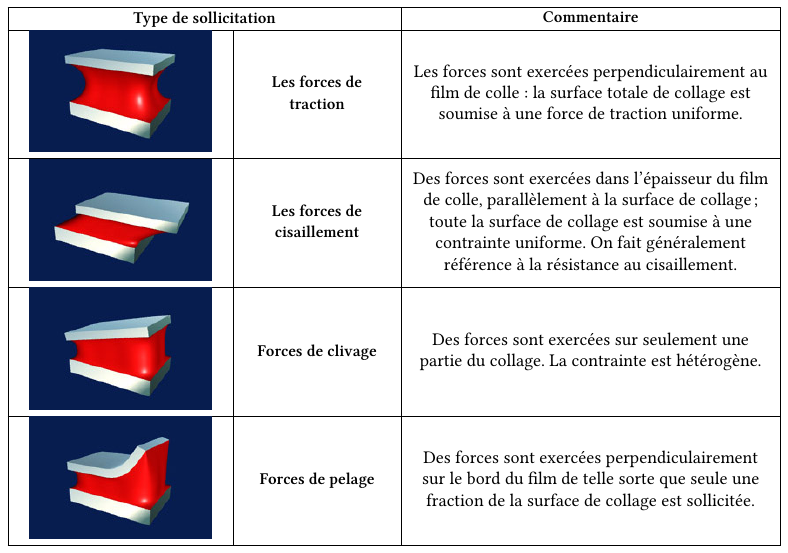
\includegraphics[width=15cm]{../Images/colle_contraintes.png}
\end{center}

La contrainte de pelage ici est la pire car elle exerce le maximum d'effort sur un très petite zone de collage ce qui amène a un déchirement du collage qui fragilise les zone voisine de collage. Pour remedier à ce problème, il faut changer de type de contrainte, dans notre cas passer d'un pelage à un cisaillement. Ceci est réalisé en collant la jointure sur la un des côté du ballon, formant ainsi un collage plat au lieu d'une forme en T.

\begin{center}
 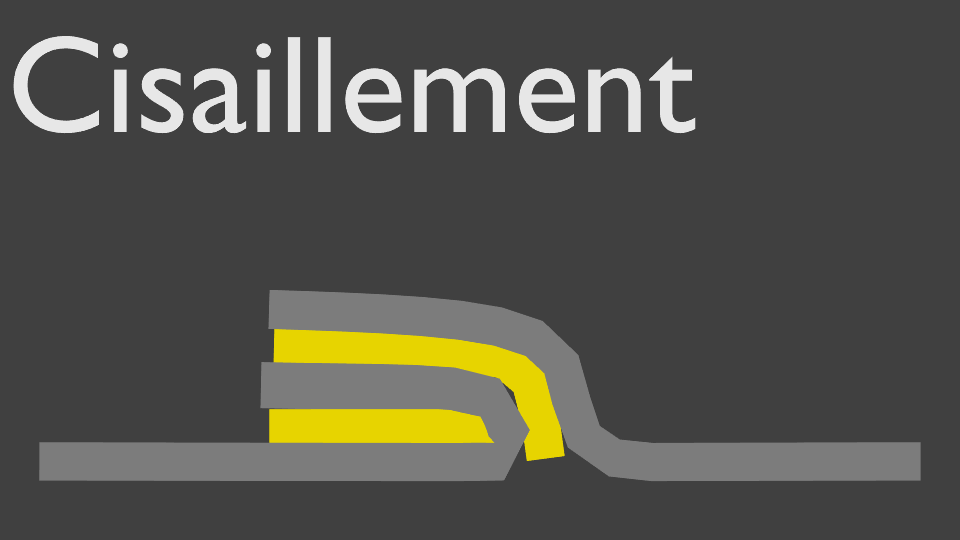
\includegraphics[width=7cm]{../Images/colle_cisaillement.png}
 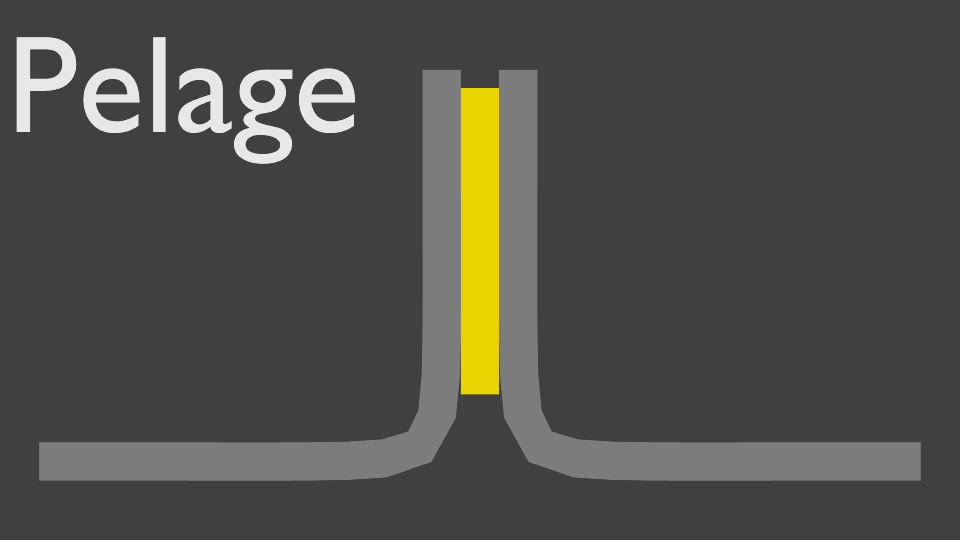
\includegraphics[width=7cm]{../Images/colle_pelage.png}
\end{center}

Deux tests de traction on alors était produit en pressant et collant deux feuilles de PET dans des planches en bois servant de support à la traction, ensuite les deux feuilles de PET étaient collé entre elle avec chacune des technique de collage.

\begin{center}
 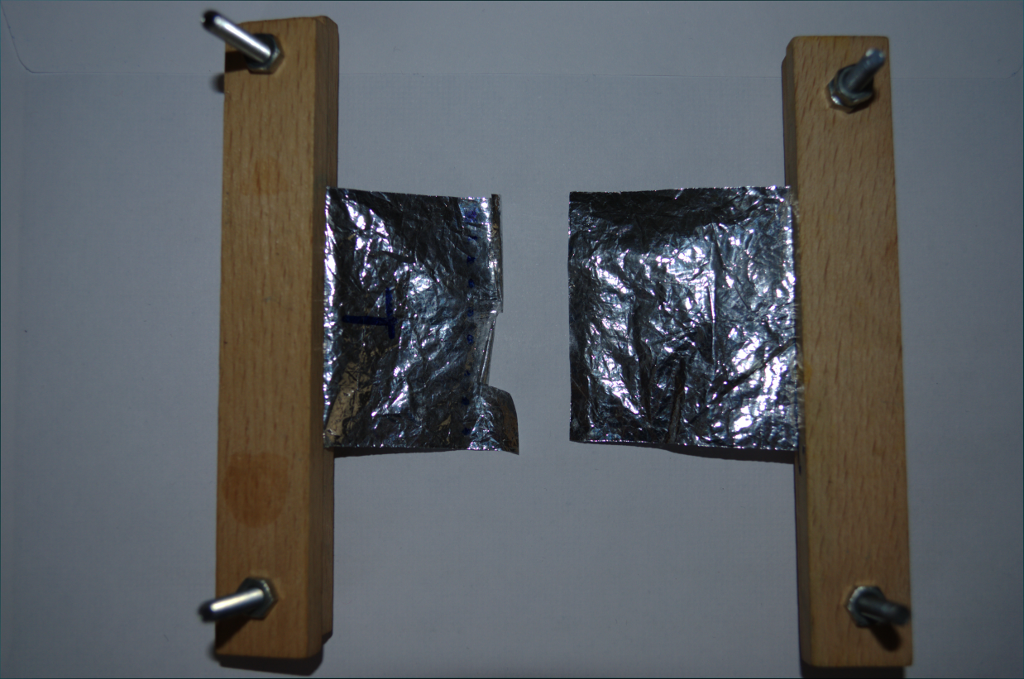
\includegraphics[width=7cm]{../Images/test_pelage.png}
 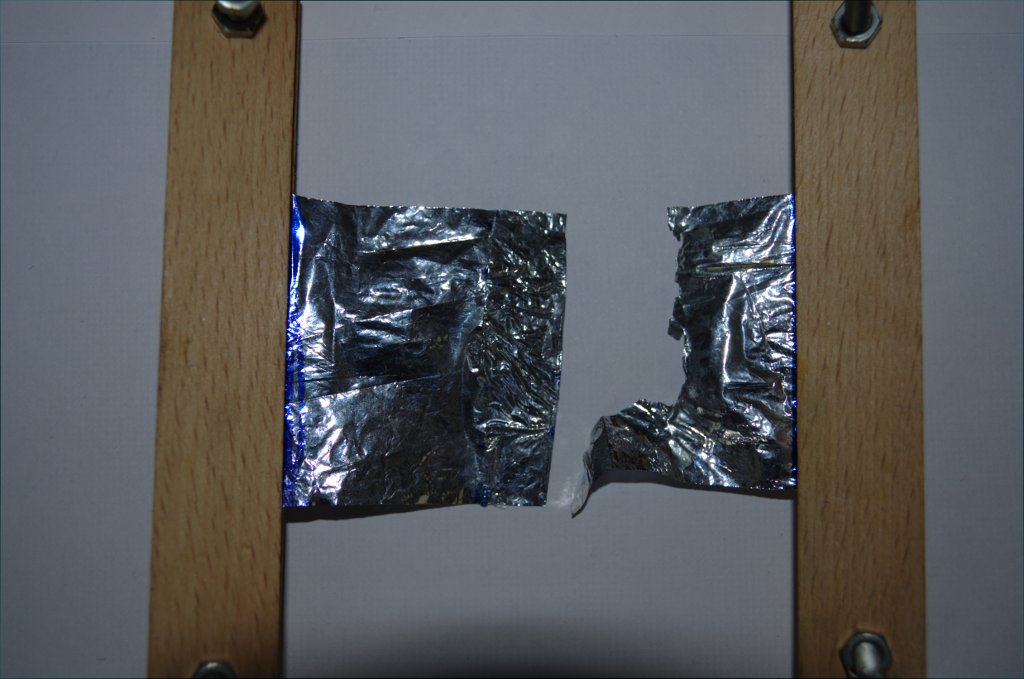
\includegraphics[width=7cm]{../Images/test_cisaillement.png}
\end{center}

% A finir.

\subsection{Forme}

Le tropodrone est composée de trois ballon de taille indentique dans le but d'avoir un centre de gravité confondus entre le drone et la structure, ce choix sera détaillé dans la partie montrant la conception de la structure.
La disposition la plus optimisée pour trois ballons est en triangle autour du drone, les ballons ressembleront donc à des parallépipède avec des pyramides à chacun de leurs sommets pour assurer une jointure entre les ballons.

\begin{center}
 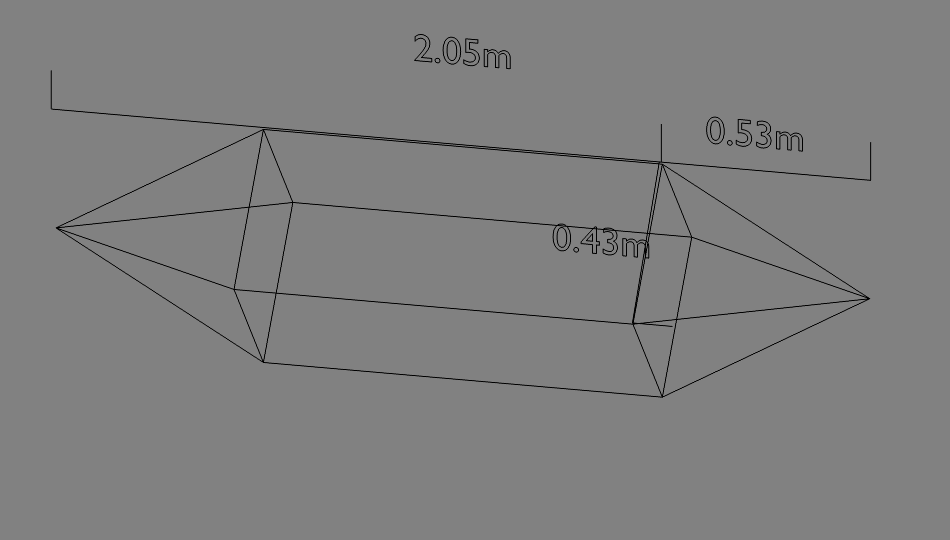
\includegraphics[width=8cm]{../Images/ballon.png}
\end{center}

\subsubsection{Calcul de la forme}

D'après le bilan maximale des masses il faudrait contenir $0.75m^3$ d'helium dans l'ensemble des ballons. Nous partons donc de l'équation du volume pour retrouver les dimensions du ballon, heureusement des contraintes sont déjà présentes~:

\begin{itemize}
 \item la longueur du parallépipède central est de 1m~;
 \item l'angle entre les arrètes du sommets de la pyramide et la base de la pyramide est de $60 \degree$~;
 \item le volume du ballon est de $0.25m^3$.
\end{itemize}

\bigbreak

Pour $b$ la largeur du ballon, la formule du volume d'un ballon se compose du volume d'un parallépipède d'un mètre~:

\begin{center}
 \boxed{V_{pa} = b^2}
\end{center}

Les deux pyramides ont un angle de $60 \degree$, leur hauteur est donc~: $\displaystyle{h = bidiagonale \times \tan{\frac{\pi}{3}}}$, où $\displaystyle{bidiagonale = \frac{\sqrt{b^2 \times 2}}{2}}$ la moitié de la diagonale de la base de la pyramide. \\
Le volume d'une pyramide est donc~:

\begin{center}
 \boxed{V_{py} = b^2 \times \frac{h}{3}}
\end{center}

La formule du volume d'un ballon est la suivante~:

\begin{center}
	\boxed{\displaystyle{V = 2(\frac{\sqrt{2 \times b^2}}{2} \times \tan \frac{\pi}{3} \times \frac{1}{3} \times b^2) + b^2}} \\
\end{center}

Nous simplifions la formule jusqu'à trouver un polynome nous facilitant la résolution pour une valeur nulle~:

\begin{center}
  $\displaystyle{V = \frac{\sqrt{6}}{3} \times b^3 + b^2 }$ \\
  $\displaystyle{b^3 \frac{\sqrt{6}}{3} + b^2 - 0.25 = 0}$
\end{center}

Malheureusement ce polynome est du troisième degrée, nous ne pouvons pas le résoudre aussi facilement qu'un polynome du second degrée, la methode la plus simple dans notre cas est d'utiliser le théorème des valeurs intermédiaires, notre fonction de volume est croissante (monome de plus haut degrée positif), continue et passant par zéro.

\begin{tikzpicture}[scale=1.5]
  \begin{axis}[
		domain=-0.1:.6,
    xlabel=$b$,
    ylabel={$V = 2(\frac{\sqrt{6}}{3} \times b^3) + b^2$},
    ytick={0, 0.25, 0.5, 0.75},
    xtick={0, 0.25, 0.43, 0.5}
  ]
		\addplot {((sqrt(6)/3) * x^3) + x^2};
		\draw (axis cs:-0.1,0.25) -- (axis cs:0.43,0.25);
		\draw (axis cs:0.43,0) -- (axis cs:0.43,0.25);
\end{axis}
\end{tikzpicture}

\paragraph{Résolution par bisection}

Pour trouver la largeur souhaité pour un volume de $0.25m^3$ nous utilisons une résolution par bissection exécuté par un programme python. Une bissection est une méthode échantillonant une fonction continue croissante ou décroissante dans un interval donné. Pour chaque interval un echantillon de la valeur intermédiare est calculé, si sa valeur est supérieur à la valeur souhaité, la borne supérieur de l'interval est réduite jusqu'à la valeur intérmédiare, dans la cas contraire où la valeur intermédiare est plus petite que la valeur souhaité, la borne inférieur de l'interval est augmenté jusqu'à la valeur intérmédiare. Chacune des modifications d'interval en crée un nouveau deux fois plus petit.
\medbreak
Le programme python procédant à cette bisection est le suivant~:

\lstset{language={Python}}
\lstinputlisting{../Ballons/Programmes/diametreBallonLatex.py}



\subsection{Structure}

\subsubsection{Étude des mouvements}

\subsubsection{Support ballon}

\subsection{Support drone}

\paragraph{1er modèle}

\paragraph{2ème modèle}

\newpage

\section{Aérodynamisme}
	Notre but a été dans cette partie de chercher une solution technique permettant de réduire la force de traînée que le drone subira quand il se déplacera, et quand il subira l'effet du vent. \\
	Il nous manquait de nombreuses notions en aérodynamisme, que nous avons pû rapidement acquérir grâce au TPE d'élèves de notre classe qui ont fait un remarquable travail sur le sujet, et grâce à un professeur de Prépa qui nous a consacré un peu de son temps.\\
	Nous les remercions ici.
\subsection{Équation de trainée}
	\begin{center}
		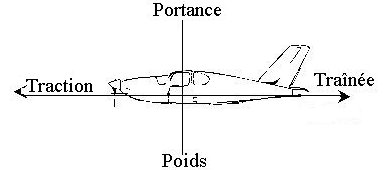
\includegraphics[width=5cm]{../Images/portance.jpg}
	\end{center}
	La force de traînée, qui représente la résistance au mouvement, est matérialisée par l'équation~:\\
  \begin{center}
   \boxed{\displaystyle{F = \frac12 \times \rho \times S \times Cx \times V^2}}
  \end{center}
  Avec~:
  \begin{itemize}
   \item $\rho$ la masse volumique du fluide dans lequel a lieu le déplacement en $kg.m^{-3}$~;
   \item S la surface soumise au flux d'air~;
   \item Cx le coefficient de traînée~;
   \item V la vitesse relative du mobile par rapport au fluide en $m.s^{-1}$.
  \end{itemize}

		Notre travail a donc été de déterminer Cx afin de résoudre l'équation.
\subsection{Optimisations techniques}
\subsubsection{Problème des ballons}
	3 ballons de 0.25 m³ créent une surface soumise au flux d'air conséquente.\\
	De plus, suivant la position des ballons, le coefficient Cx sera plus ou moins conséquent.\\
	\\
	Il nous faut donc trouver une forme favorable, c'est à dire réduisant la surface et ayant un faible coefficient de traînée.

\subsubsection{La forme en triangle}
	La forme en triangle que nous vous avons présenté précédemment (LIEN CHAP. STRUCTURE) présente de nombreux avantages.
	\\
	Le premier est qu'elle permet de créer un couloir dans lequel le vent s'engouffre ; cette forme permet de réduire la force de traînée et a l'avantage de ne présenter aucune position dans laquelle le vent aurait un trop grand effet.
	De plus, nous avons trouvé une solution technique permettant de profiter de ce couloir d'air le plus souvent possible : installer un gouvernail.
\subsubsection{Gouvernail}
	\begin{center}
		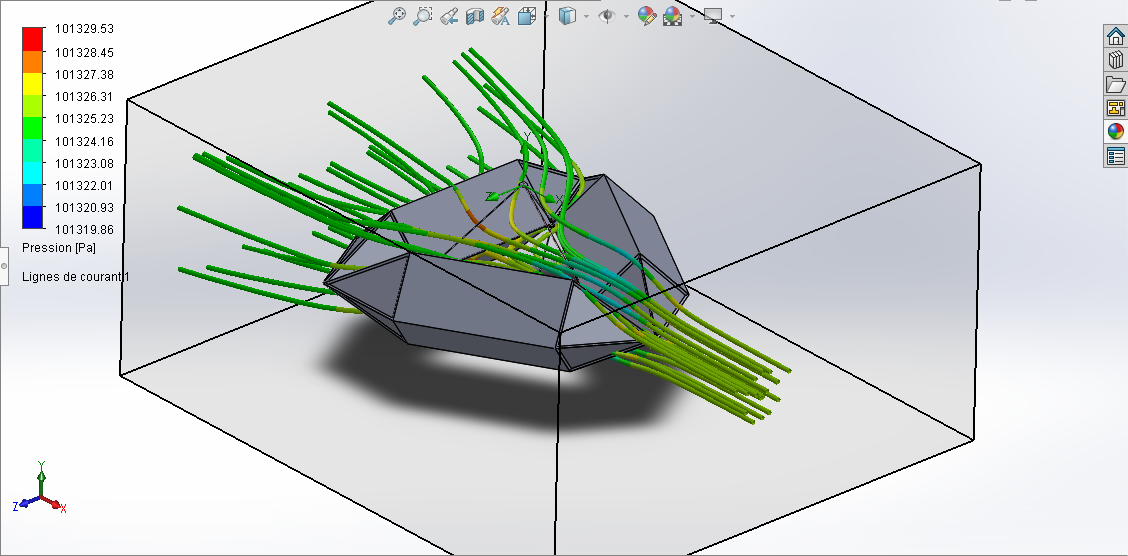
\includegraphics[width=14cm]{../Images/Capture.PNG}
	\end{center}
	Le gouvernail nous permet d'orienter les ballons en fonction de la direction du drone, ce qui force la structure a garder une position théoriquement plus favorable que les autres.
	Nous pouvons faire une analogie avec les différentes conformations d'une molécule : le gouvernail nous permet de garder la position la moins dépensière d'énergie.\\
	\\
  Cette solution a toutefois un désavantage : elle réduit la manoeuvrabilité immédiate du drone en faisant apparaître une force supplémentaire. Toutefois, nos calculs montreront que cette force est négligeable en comparaison du gain sur de longues distances.


\subsection{Calcul du Cx}
\paragraph{Pour une sphère}
	Nous avons dans un premier temps essayé de calculer le Cx à la main, en prenant la seule approximation dont nous avions les données : le Cx d'une sphère.\\
	Celui-ci se calcule en fonction du nombre de Reynolds, qui définit le type d'écoulement auquel est soumis la structure :
	\begin{center}
   \boxed{\displaystyle{Re = \frac{V \times L}{\nu}}}
  \end{center}
	Avec~:
  \begin{itemize}
	 \item $\rho$ la masse volumique du fluide dans lequel a lieu le déplacement en $kg.m^{-3}$~;
   \item V la vitesse relative du mobile par rapport au fluide en $m.s^{-1}$;
   \item L la dimension caractéristique (ici le diamètre de la sphère)~;
   \item $\micro$ la viscosité cinématique du fluide~;
  \end{itemize}
	Nous avons réalisé grâce à cette formule un algorithme python permettant de calculer la force de traînée du ballon.\\
	\\
	Toutefois, cette approximation n'était pas vraiment précise, et n'ayant pû mettre la main sur la soufflerie, nous nous sommes rabattus sur Solidworks et sur son module complémentaire FlowSimulation.
\paragraph{Simulation SW}
	L'avantage de Solidworks est qu'il est très précis et qu'il est facile de déterminer le Cx dans plusieurs positions.\\
	\begin{center}
		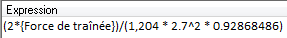
\includegraphics[width=15cm]{../Images/expressionCX.png}
		\captionof{figure}{Objectif de calcul pour déterminer Cx.}
	\end{center}

\subsubsection{Simulation tableur et équation}
	La simulation a été réalisée plusieurs fois dans plusieurs positions selon l'axe Z.\\
	Ces données ont été rentrées dans un tableur, et nous ont permis de confirmer l'intérêt du gouvernail.\\
	\\
	Nous avons également pû relever la force théorique maximale auxquel le drone peut être soumis.\\
	(...)
\subsection{Vitesse de vent maximum}
	Chaque moteur fournit 2 N.\\
	(...) TRIGO ().
\section{Réalisation}
\begin{center}
	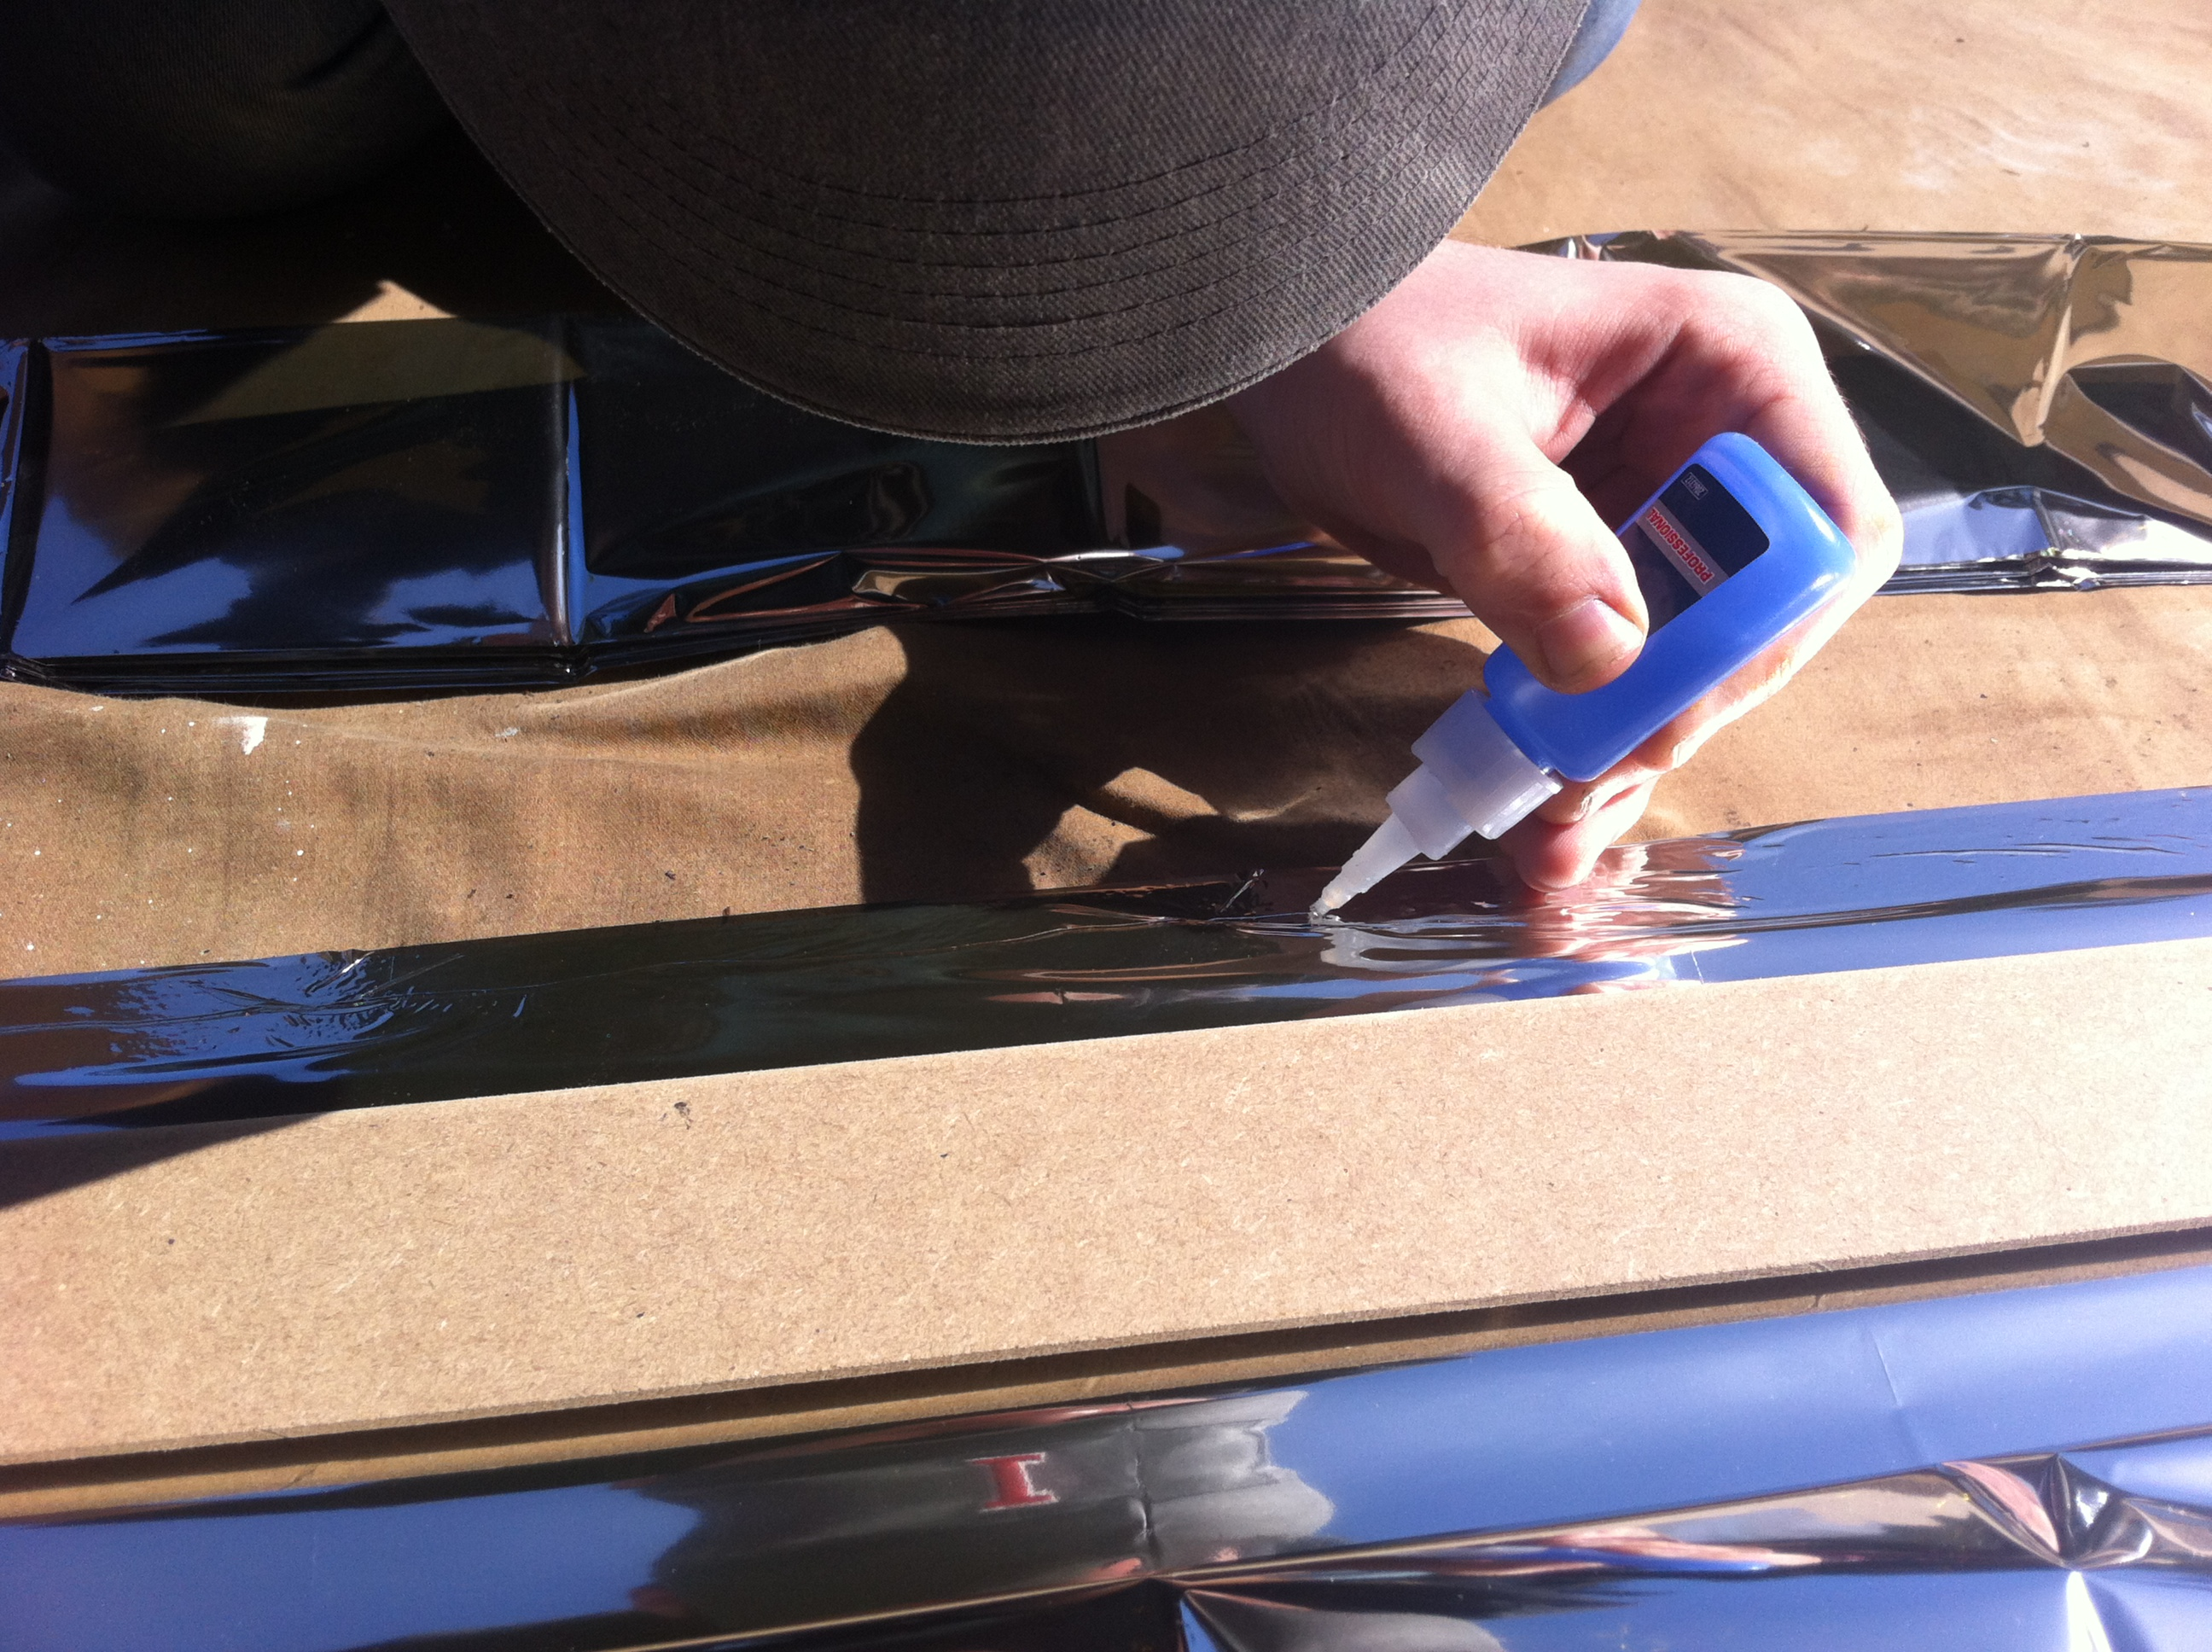
\includegraphics[width=15cm]{../Images/assen_1.JPG}
\end{center}
\begin{center}
	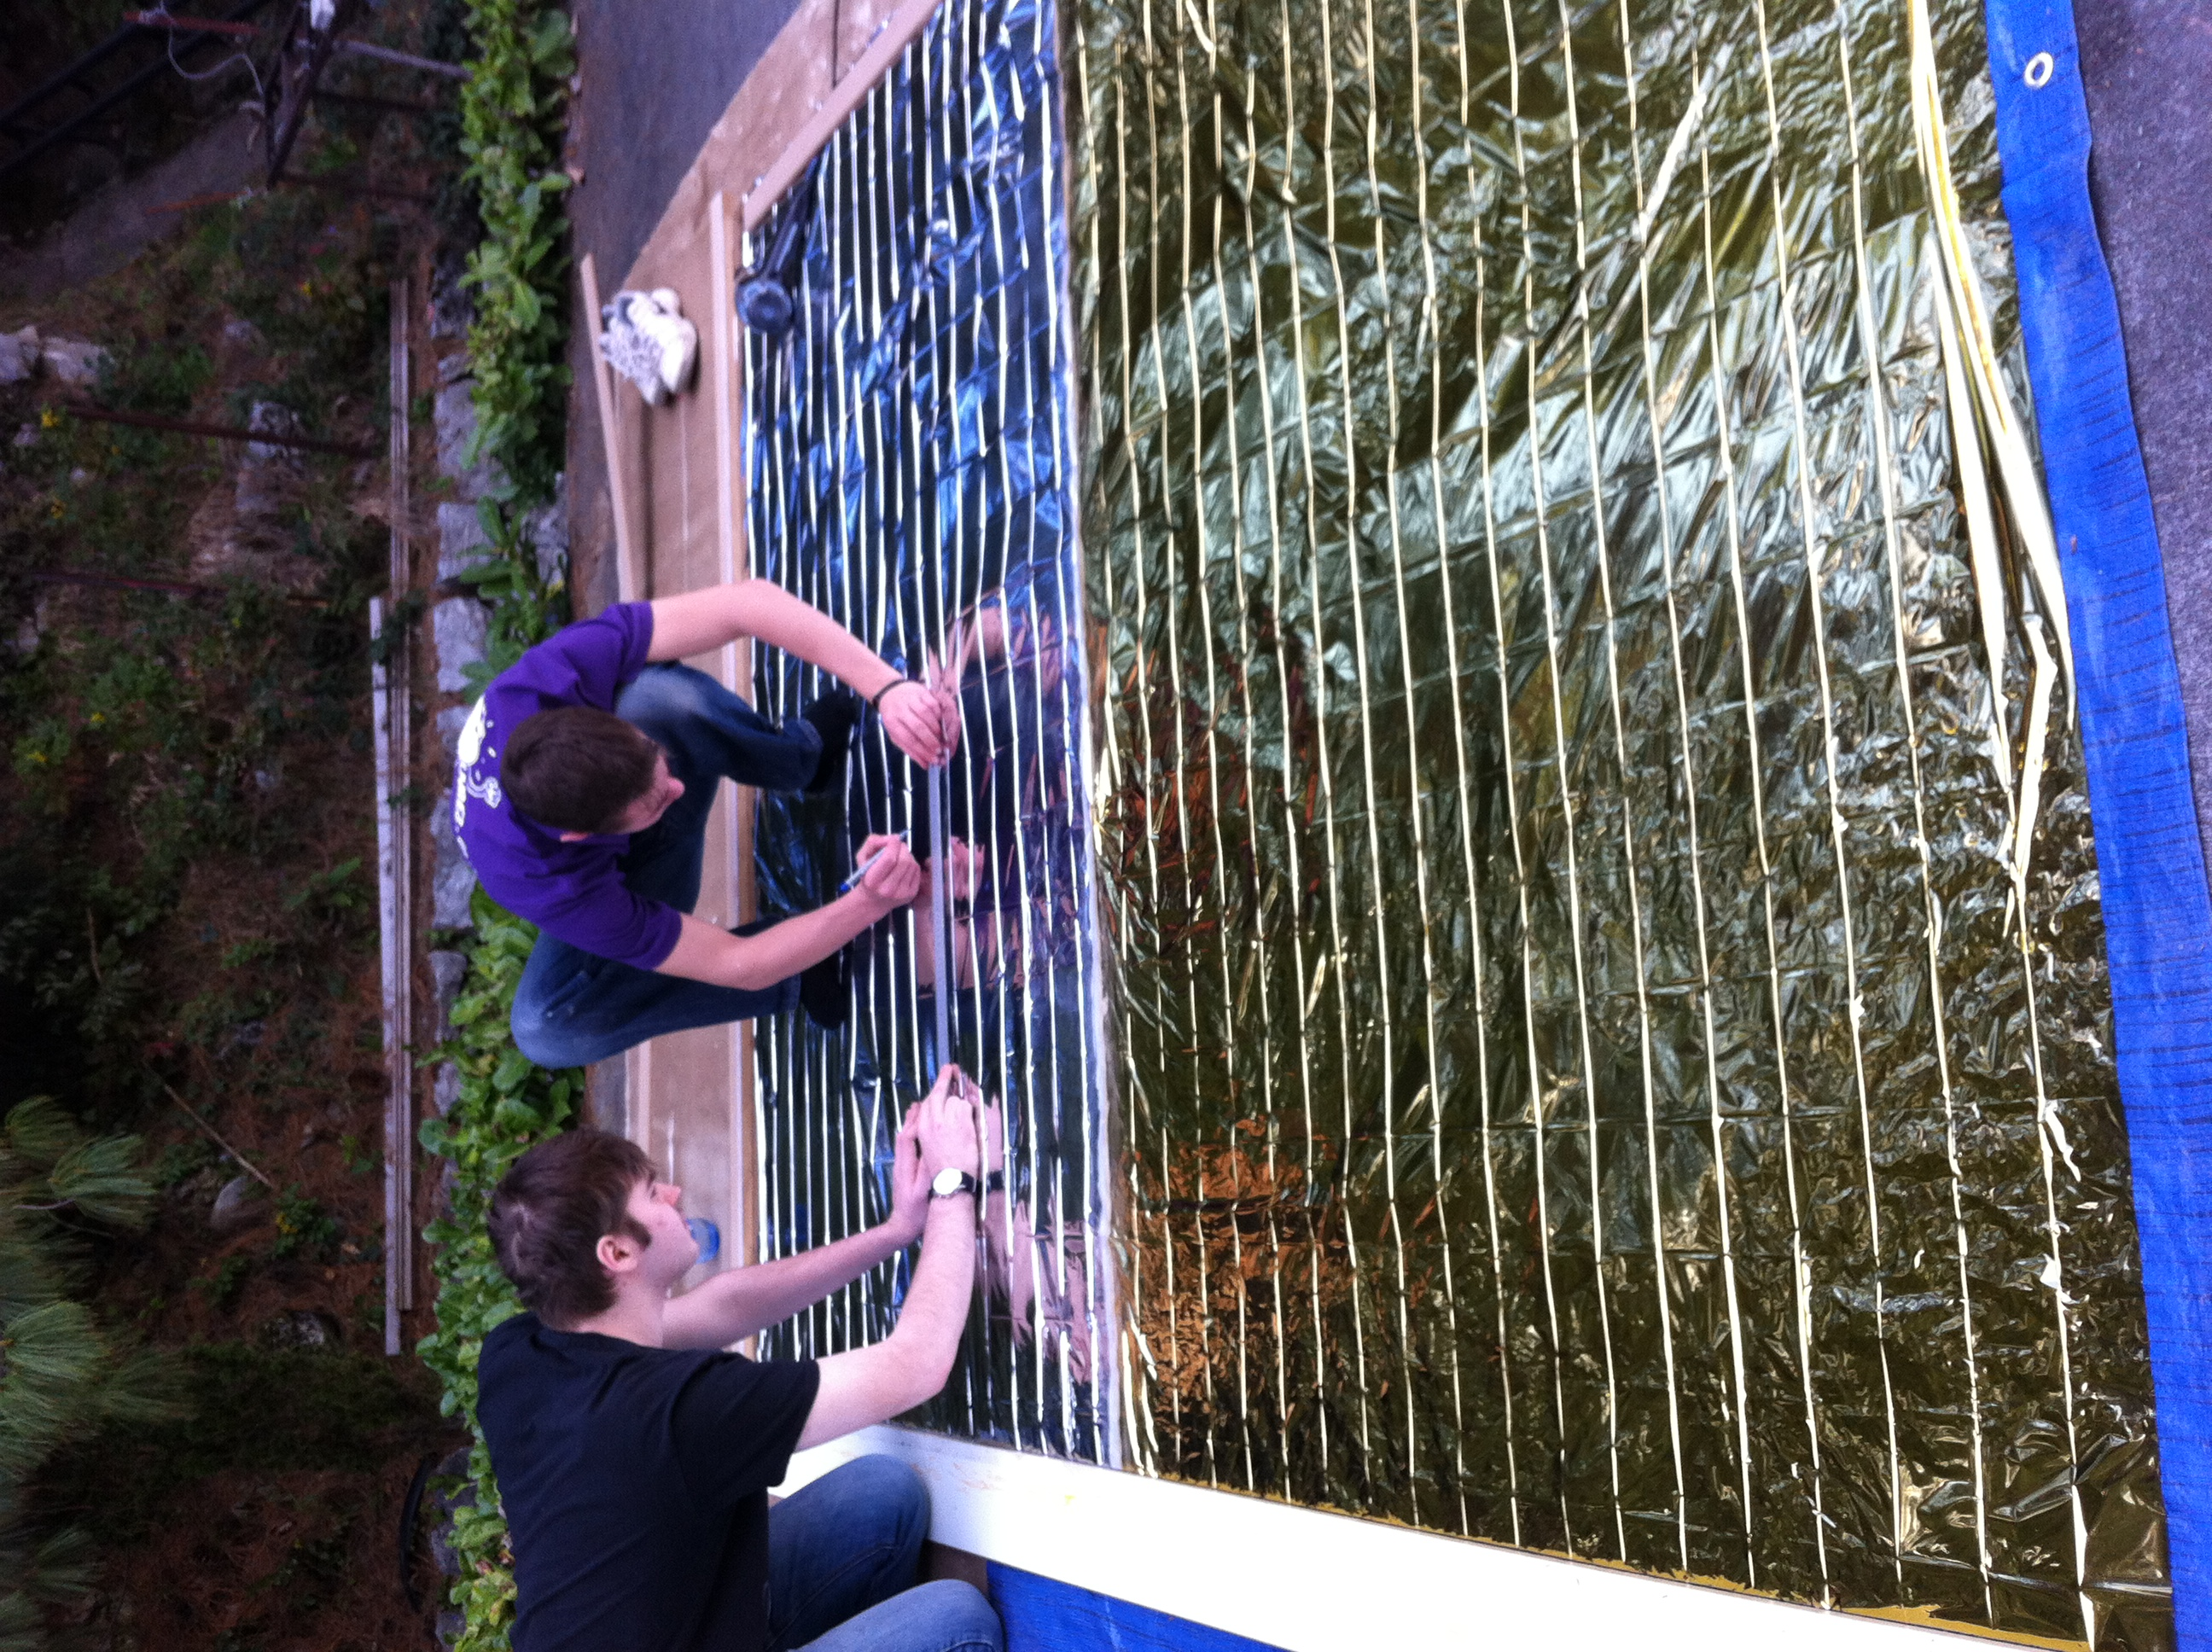
\includegraphics[width=15cm]{../Images/assen_2.JPG}
\end{center}
\begin{center}
	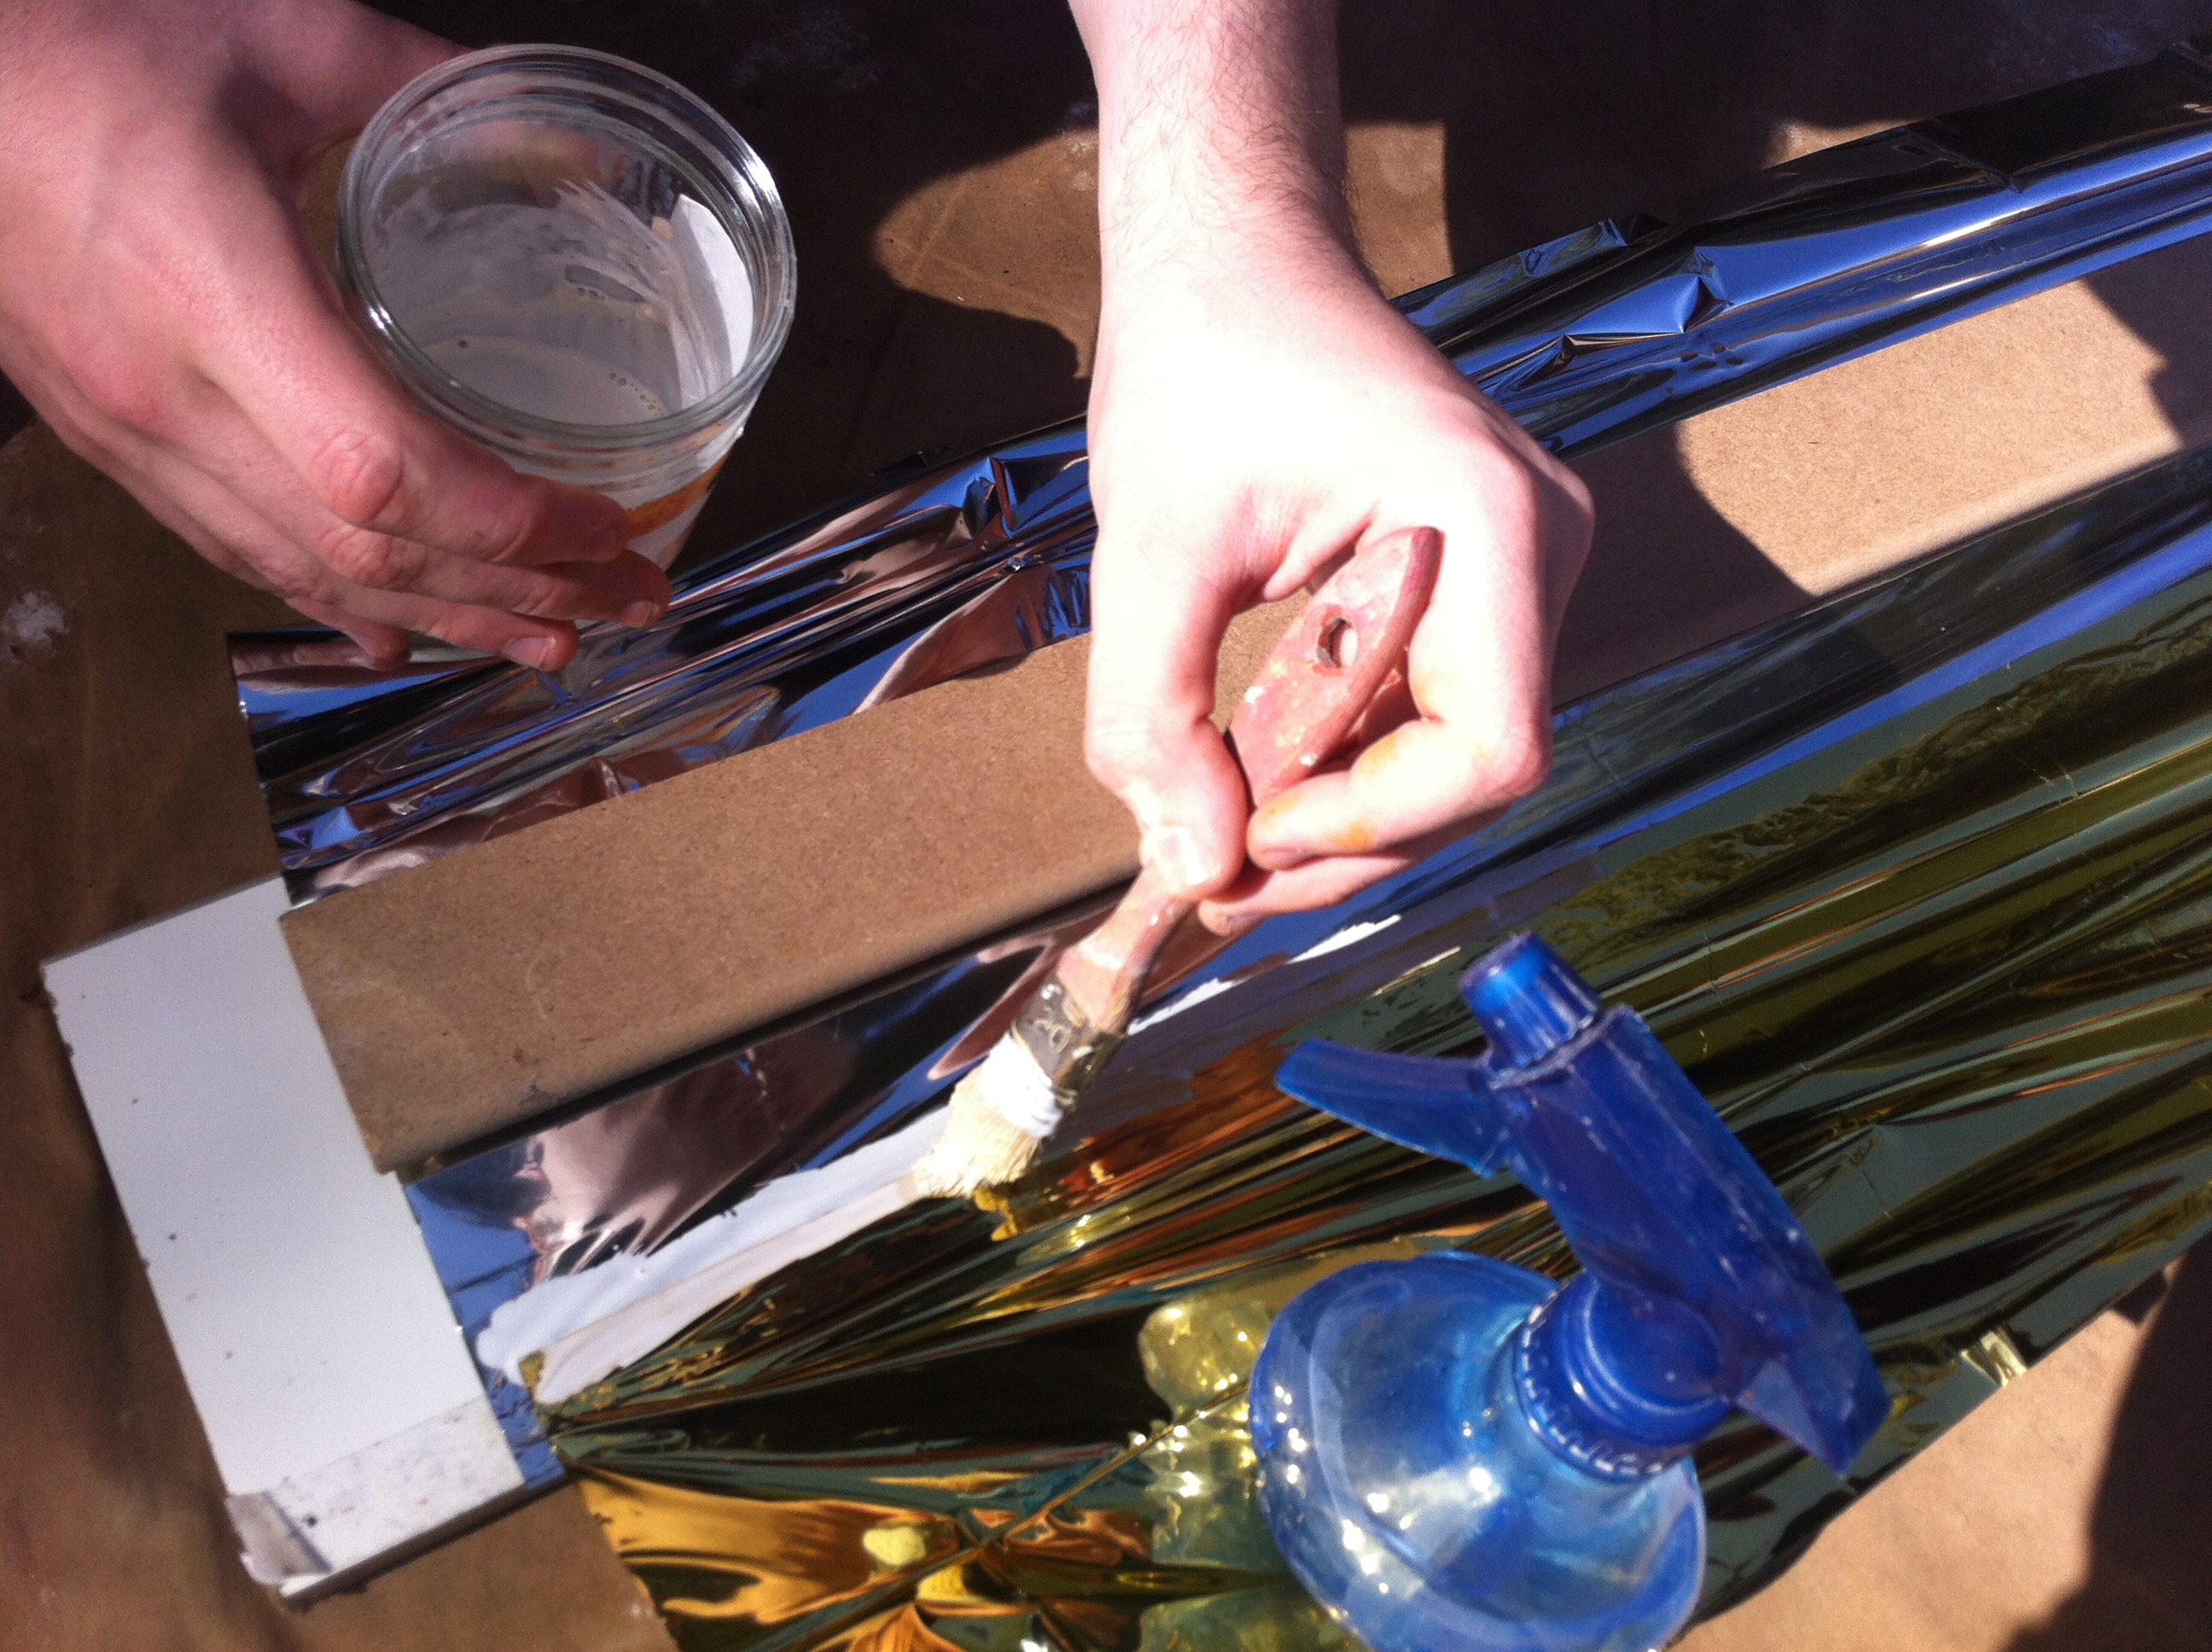
\includegraphics[width=15cm]{../Images/assen_3.JPG}
\end{center}

\end{document}
